\section{Discussion and Conclusion}
\label{c4:sec-concl}
%\textit{This chapter discusses}
\vspace{2ex}\vfill

\subsection{Discussion about abstract traces}
%{\color{blue}XXX Cette discussion doit être un lien vers la 3e partie.à mettre dans la conclusion?? }

One way to bypass the problem raised by  multimedia applications in which raw execution traces are very large (more than a gigabyte for few minutes of video decoding \cite{guerin10,prada10}) is to abstract traces. The abstraction process produce more
 compact traces and facilitate the readability of traces for human programmers.
An abstract trace example is given Fig. \ref{fig-abs}.\\


\begin{figure}[h!]
 \begin{center}
 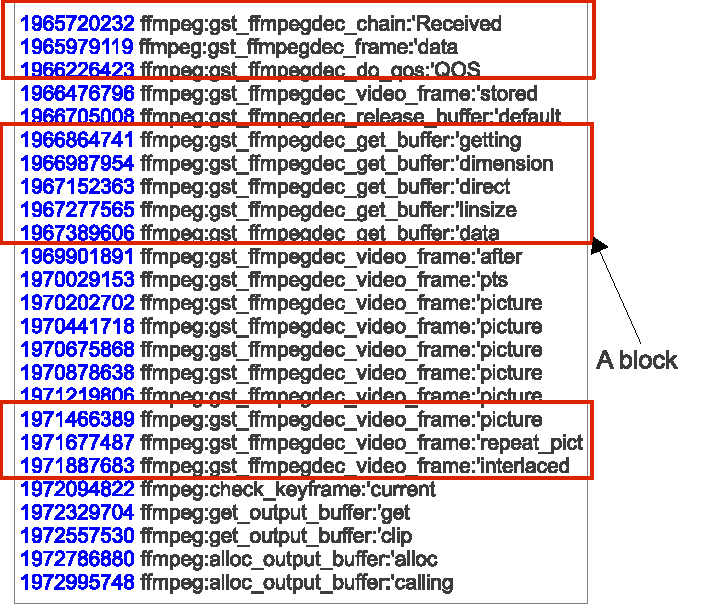
\includegraphics[scale=0.55]{chap4/images/trace-eps-converted-to.pdf}
\end{center}
\caption{A block in an execution trace}
\label{fig-EAA}
\end{figure}

We define as \textit{timestamped block} a pair $(t,B)$ where $B$ is a block and $t \in \mathbb{N}$,  is the timestamp of the first event of $B$. 
A \textit{abstracted trace} is a sequence of timestamped blocks.
The length of a abstracted trace $T$ denoted $|T|$ is the number of its blocks (c.f. fig. \ref{fig-EAA}). 
 The size of a sequence $S$, denoted by $\|S\|$, is the total number of events that it contains. For an execution trace $T$, $|T|=\|T\|$ whereas for an abstracted trace $T^a$, described by blocks,  $|T^a| \neq \|T^a\|$ (except when blocks are singletons of events).

\begin{figure*}[h!pbt]
\centering
 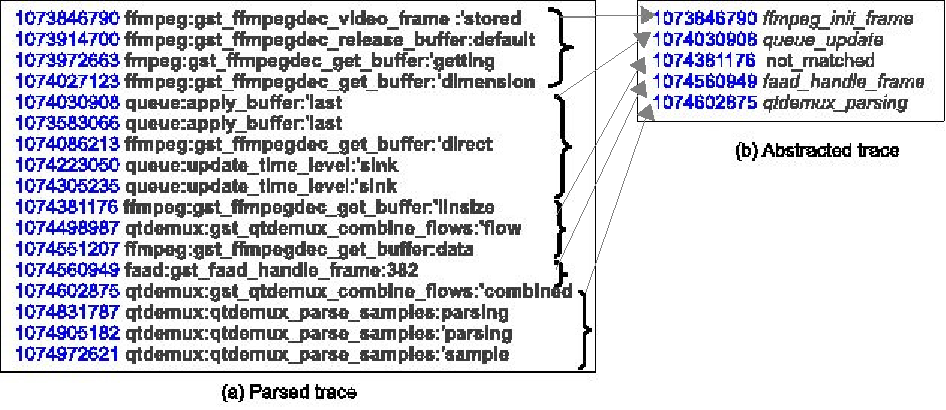
\includegraphics[scale=0.63]{chap4/images/expe_trace2-eps-converted-to.pdf}
\caption{An abstracted trace obtained with {\em FrameMiner}}
\label{fig-abs}
\end{figure*}
 Fig \ref{fig-abs} is an example of abstracted trace obtained by {\em FrameMiner} \cite{ck2013} on \textit{pub} video.

Our approach gains to be generic i.e. applicable to execution traces described at different levels of abstractions: on raw execution traces that are sequences of time-stamped low-level events, as well as on sequences of time-stamped \emph{blocks}, in which (subsequences of) low-levels  events have been abstracted into blocks \cite{ck2013}
 more meaningful to the programmer. In order to apply TED on abstract traces, a first idea would be to consider occurrence of a block as a strict sequence of events and to apply our distances not on events but on blocks. The adaptation of TED to abstracted traces is currently under development.\\
%In discussion, talk about the possibiliy of semantics


% Parler du fait que c'est une sorte de distance++ car on a les valeurs mais aussi le pb => semantique
%Ainsi parler du fait que le debugging de trace est en général basé sur la visualisation
%Parler des distances applicables sur les séquences.
%Further work sur l'utilisation d'une ontologie avec la nouvelle définition de l'opérateur d'égalité?P3
%discussion sur l'application des distances sur traces abstraites??


%**************************Related Work**********************************************
%\textbf{Distances measures for sequences:} An important issue in measuring similarity/distance between two sequences is the ability to deal with outlying points, noise in the data, amplitude differences and the existence of gaps and other time axis distorsion problems \cite{outsurvey11}. 
%************************Conclusion***************************************************
\subsection{Concluding Remarks}
To analyse traces of finished events, and fix bugs, programmers use several tools such as trace visualizers (\cite{paje,tracevis,vet,surv08})
 and techniques such as tracepoints on the execution traces. These techniques need to have an expert to 
interpret the graphical representation. In contrast, our work based on distances develops a technique which limits the developer intervention.

There is an abundant literature about distances. For distances between sequences, an edit distance model is used in \cite{do09} 
to approximate matching of timed strings; \cite{kos11, gu12} propose to represent each sequence in a suitable form, before computing distance. 
However, very few distances take into account the temporal aspect. We propose a temporal distance that is adapted for trace comparison. But the 
most distinguishing point of our approach is that our method is the first, to the best of our knowledge which returns a diagnosis to the user, 
added to the effective values of distance.

Our approach diagnoses anomalies in an execution trace of multimedia application, by comparison with a reference trace. We use distances as models 
of comparison and specifically design three distinct distances in order to tackle well-known anomalies of the multimedia domain. We experimentally 
show the originality of our solution compared to existent distances and show that our proposed approach scales well to real huge application traces. 
Distances defined in our approach allow to identify a specific problem and give a semantic added-value level to the analysis. Moreover, as all 
distances, they also provide insights of how far an abnormal trace is from a correct one. We also present a use case on how TED performs the 
analysis of a trace and conduct some experiments to evaluate TED scalability and accuracy. 

Our general approach is similar to hypohetico-deductive model \cite{hypodeduc1}, which is a form of deductive reasoning that begins with general principles
, assumptions, and ideas, and works from them to more particular statements about what world actually looks like and how it works. The hypotheses are then tested by gathering and analyzing 
data and the theory is then either supported or refuted by the results \cite{hypodeduc2}. We formulated the hypothesis of well known anomalies, we observed data 
and made corresponding statements to detect anomalies.

We have three research directions. The first direction is to adapt our distances to abstract traces so that our proposal be as generic as possible. 
The second direction is to enlarge TED to other types of anomalies for instance the image is completely fuzzy, upside down and/or cut in half. 
The strength of our contribution is that it is easily extensible  to other types of anomalies. For each new anomaly, we only need to follow the 
same methodology as explained in this part to find the best suitable distance able to clearly detect the anomaly. There is no need to do any changes
 in TED existing architecture.  Finally, additional constraints can be introduced such as parallel execution traces and 
the challenge is to identify, for example, streams of different execution and take them into account for the computation of distances.

%\cite{cha07,cha10} provides surveys of binary distances and distances based on  probability density functions. 

% Conclusion et perspectives ; c’est un résumé étendu ; rappeler le problème, les résultats connus avant la partie et la nouvelle solution proposée ; 
% donner une évaluation explicite du chemin parcouru par rapport à l'objectif annoncé dans l'introduction ; les perspectives doivent découler directement
%  et de manière naturelle du travail réalisé ; si la solution proposée n'est pas optimale, alors proposer des pointeurs pour l’exploration de meilleures
%  solutions ; si la solution est optimale alors donner des perspectives liées plutôt à la résolution d’autres problèmes connexes ou plus généraux.

